%
% Book intro pages (frontmatter)
%
\maketitle
\begin{center}
Κάθε γνήσιο αντίτυπο φέρει την υπογραφή του συγγραφέα:
\begin{tabular}{p{0.9\textwidth}}
\\
\\
\\
\end{tabular}

\bigskip
1η Έκδοση -- Χανιά, XX/XX/2017

[ Αριθμός αντιτύπου: 1 ]

\bigskip
Copyright \copyright 2008 -- 2016 Μανώλης Κιαγιάς

Το Έργο αυτό διατίθεται υπό τους όρους της Άδειας:\\

\includegraphics[scale=0.2]{images/license/cc-logo}\\
\textbf{Αναφορά -- Μη Εμπορική Χρήση --  Παρόμοια Διανομή 3.0 Ελλάδα}\\
Μπορείτε να δείτε το πλήρες κείμενο της άδειας στην τοποθεσία:\\
\url{http://creativecommons.org/licenses/by-nc-sa/3.0/gr/}
\end{center}
\subsection*{Είναι Ελεύθερη:}

\noindent
\textbf{Η Διανομή} -- Η αναπαραγωγή, διανομή, μετάδοση και παρουσίαση του Έργου σε κοινό

\subsection*{Υπό τις ακόλουθες προϋποθέσεις:}

\vspace{1em}
\noindent
\parbox{1.5cm}{
\includegraphics[scale=0.15]{images/license/cc_by_30}}
\parbox{10.5cm}{\textbf{Αναφορά Προέλευσης} — Θα πρέπει να αναγνωρίσετε την προέλευση στο έργο σας με τον τρόπο που έχει ορίσει ο δημιουργός του ή το πρόσωπο που σας χορήγησε την άδεια (χωρίς όμως να αφήσετε να εννοηθεί  ότι εγκρίνουν  με οποιονδήποτε τρόπο εσάς ή τη χρήση του έργου από εσάς).}

\vspace{1em}
\noindent
\parbox{1.5cm}{
\includegraphics[scale=0.15]{images/license/cc_nc_30}}
\parbox{10.5cm}{\textbf{Μη Εμπορική Χρήση} --  Δεν μπορείτε να χρησιμοποιήσετε αυτό το έργο για εμπορικούς σκοπούς.}

\vspace{1em}
\noindent
\parbox{1.5cm}{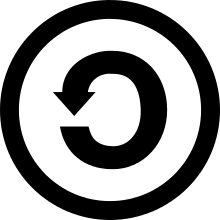
\includegraphics[scale=0.15]{images/license/cc_sa_30}}
\parbox{10.5cm}{\textbf{Παρόμοια Διανομή}  — Αν αλλοιώσετε, τροποποιήσετε ή δημιουργήσετε κάποιο παράγωγο έργο το οποίο βασίζεται στο παρόν έργο, μπορείτε να διανείμετε το αποτέλεσμα μόνο με την ίδια ή παρόμοια με αυτή άδεια.}

\subsection*{Με την κατανόηση ότι:}

\noindent
\textbf{Αποποίηση} -- Οποιεσδήποτε από τις παραπάνω συνθήκες μπορούν να παρακαμφθούν αν πάρετε την άδεια του δημιουργού ή κατόχου των πνευματικών δικαιωμάτων.

\vspace{1em}
\noindent
\textbf{Άλλα Δικαιώματα} -- Σε καμιά περίπτωση τα ακόλουθα δικαιώματα σας, δεν επηρεάζονται από την Άδεια:

\begin{itemize}
  \item Η δίκαιη χρήση και αντιμετώπιση του έργου
  \item Τα ηθικά δικαιώματα του συγγραφέα
  \item Τα ενδεχόμενα επί του έργου δικαιώματα τρίτων προσώπων, σχετικά με τη χρήση του έργου, όπως για παράδειγμα η δημοσιότητα ή ιδιωτικότητα.
\end{itemize}

\vspace{1em}
\noindent
\textbf{Σημείωση} -- Για κάθε επαναχρησιμοποίηση ή διανομή, πρέπει να καταστήσετε σαφείς στους άλλους τους όρους της άδειας αυτού του Έργου. Ο καλύτερος τρόπος να το πράξετε αυτό, είναι να δημιουργήσετε ένα σύνδεσμο με το διαδικτυακό τόπο της παρούσας άδειας:
\begin{center}
\url{http://creativecommons.org/licenses/by-nc-sa/3.0/gr/}
\end{center}
\line(1,0){275}\\\\
\begin{tabular}{p{0.95\textwidth}}
Το βιβλίο αυτό στοιχειοθετήθηκε σε \XeLaTeX{}.  Ο πηγαίος κώδικας του είναι διαθέσιμος στις δικτυακές τοποθεσίες που αναφέρονται παρακάτω και μέσω mercurial repository.\\
\end{tabular}

\bigskip
Επισκεφθείτε το δικτυακό τόπο του μαθήματος
και κατεβάστε την τελευταία έκδοση του βιβλίου και διορθώσεις:

\bigskip
\begin{center}
\url{http://diktia.chania-lug.gr}
\end{center}
\bigskip
Σε περίπτωση προβλήματος χρησιμοποιήστε το mirror site:
\bigskip
\begin{center}
\url{http://www.freebsdworld.gr/diktia/diktia2016.pdf}
\end{center}
\newpage
(Κενή Σελίδα)
\newpage
Το βιβλίο αυτό αφιερώνεται σε όσους κάνουν αυτό που πιστεύουν και όχι αυτό που νομίζουν οι άλλοι σωστό\ldots\\

\begin{figure}[!ht]
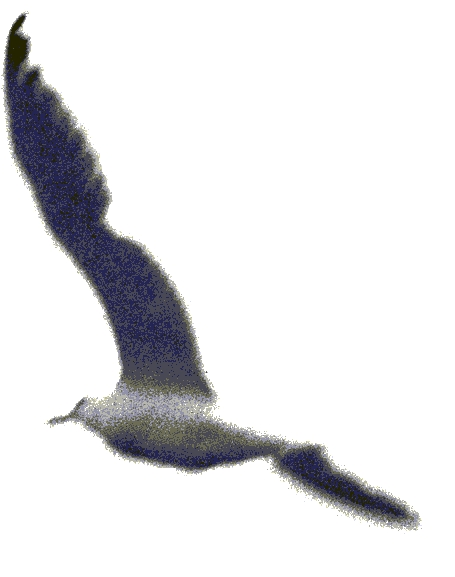
\includegraphics[width=0.9\textwidth]{images/intro/glaros}
\end{figure}
\begin{quote}
``Ο μόνος αληθινός νόμος είναι εκείνος που οδηγεί στην ελευθερία'', είπε ο Ιωνάθαν· ``Δεν υπάρχει άλλος.''

\flushright{\textit{``Ο Γλάρος Ιωνάθαν Λίβινγκστον'', Richard Bach}}
\end{quote}
\newpage
(Κενή Σελίδα)
\newpage
\section*{Εισαγωγή στο Νέο Βοήθημα}
Καλώς ήλθατε στην πρώτη έκδοση του νέου ``ανεπίσημου'' βοηθήματος για το
μάθημα ``Δίκτυα Υπολογιστών'' το οποίο διδάσκεται ως
Πανελλαδικά εξεταζόμενο στην Γ' Τάξη των Επαγγελματικών Λυκείων.  Το βιβλίο
αυτό καλύπτει την εξεταζόμενη ύλη όπως ανακοινώθηκε από το Υπουργείο Παιδείας
για το σχολικό έτος 2016-2017 σύμφωνα με το νέο σχολικό βιβλίο και το πρόγραμμα
σπουδών.  Το νέο ανεπίσημο βοήθημα, με απλοποιημένη
αλλά άρτια τεχνικά γλώσσα, ευελπιστεί να καλύψει τις ατέλειες του σχολικού
εγχειριδίου και να βοηθήσει τους αποφασισμένους μαθητές να πετύχουν στις
εξετάσεις. Η επιτυχία των δύο αρχικών βοηθημάτων για το ΤΕΕ και το ΕΠΑΛ,
μας οδηγεί να πιστεύουμε ότι ο στόχος αυτός είναι εφικτός.

Η έκδοση αυτή κυκλοφορεί ως ``ελεύθερη'' με βάση την άδεια Creative Commons
που μπορείτε να διαβάσετε στις πρώτες σελίδες του βιβλίου.

\section*{Πρόλογος της  Πρώτης Έκδοσης (2004)} 
\begin{quote}
Προλογίζει ο Αντώνης Αθανασάκης, καθηγητής στον Τομέα Οικονομίας, συνάδελφος του συγγραφέα στο ΤΕΕ Κισάμου.
\end{quote}
Κάθε απόπειρα αγωγής καταλήγει σε σχέση μεταξύ προσώπων. Η διδασκαλία, δεν είναι ενέργεια κατά την οποία επικοινωνούν μόνο οι εγκέφαλοι, αλλά πορεία προσωπικής επικοινωνίας και αμοιβαίας προσπάθειας. 

Το εγώ που δεν έχει απέναντί του κανένα συγκεκριμένο εσύ, αλλά είναι περιστοιχισμένο από μια πληθώρα ``περιεχομένων'', δεν είναι διόλου παρόν και η στιγμή του είναι στερημένη από παρουσία. Μια παρουσία όμως δεν είναι κάτι που ξεφεύγει και γλιστράει αλλά είναι εκείνο που κατοικεί απέναντί μας και περιμένει την συνάντηση. 

Αν η πραγματική συνάντηση είναι η πορεία, κατά την οποία ένας άνθρωπος αγγίζει έναν άλλον άνθρωπο στον πυρήνα του, τότε οι μαθητές του Μανώλη είχαν φέτος μια τρομερή ευκαιρία.

Το μόνο που χρειάζονται είναι την ικανότητα για ανταπόκριση. Γιατί η ελευθερία μέσα στην αγωγή, είναι το να μπεις σε δεσμό. Το αντίθετο του εξαναγκασμού, σύμφωνα με τον Buter δεν είναι η ελευθερία, αλλά ο δεσμός. Δεν θα μπορούσαμε χωρίς ελευθερία, αλλά από μόνη της δεν είναι χρησιμοποιήσιμη.
\newpage
\tableofcontents
\listoffigures
